\documentclass[12pt, twoside]{article}
\input{../preamble}
\usepackage{float}

\fancyhead[LO]{La Scuola d'Italia / Dr.\ Huson / IB Math \\* 18 May 2026}
\fancyhead[RO]{\fbox{\begin{minipage}{6cm}\footnotesize First \& Last name:\\[0.5cm]\end{minipage}}}
\fancyfoot[C]{\thepage}

\begin{document}
\subsubsection*{8.1 Classwork: Rational Functions and Asymptotes}

\begin{enumerate}[itemsep=0.4cm]

%--- Problem 1: Warmup --- explore 1/x near 0 and at large |x| ---
\item[1.] \textbf{Warmup.} Consider the function
$$f(x) \;=\; \dfrac{1}{x}.$$

\textbf{(a)} Complete the table. Give decimals to 3 significant figures
where needed.

\vspace{0.2cm}
\begin{center}
\renewcommand{\arraystretch}{1.6}
\begin{tabular}{|c|c|c|c|c|c|c|c|}
\hline
$x$       & $-1000$ & $-10$ & $-0.1$ & $-0.001$ & $0.001$ & $0.1$ & $10$ \\
\hline
$f(x)$    & \phantom{XXXXX} & \phantom{XXXXX} & \phantom{XXXXX} & \phantom{XXXXX} & \phantom{XXXXX} & \phantom{XXXXX} & \phantom{XXXXX} \\
\hline
\end{tabular}
\end{center}
\vspace{0.3cm}

\textbf{(b)} Describe what happens to $f(x)$ as $x$ approaches $0$
from the right (positive side), and as $x$ approaches $0$ from the
left (negative side).

\vspace{2.0cm}

\textbf{(c)} Describe what happens to $f(x)$ as $x$ becomes very
large (positive), and as $x$ becomes very large negative.

\vspace{2.0cm}

\textbf{(d)} Sketch the graph of $f$ on the axes below. Write down the equations of the vertical asymptote and the horizontal asymptote of $f$.

\vspace{1.6cm}

\newpage

%--- Problem 2: Identify asymptotes by inspection ---
\item[2.] For each function below, write down the equation of the
vertical asymptote and the equation of the horizontal asymptote.

\begin{enumerate}[label=(\alph*), itemsep=0.6cm]
  \item $\displaystyle f(x) = \dfrac{1}{x-3}$
  \vspace{0.6cm}

  \item $\displaystyle f(x) = \dfrac{1}{x+5} + 2$
  \vspace{0.6cm}

  \item $\displaystyle f(x) = \dfrac{3}{x} - 1$
  \vspace{0.6cm}

  \item $\displaystyle f(x) = \dfrac{2}{x-4} + 1$
\end{enumerate}

\vspace{0.3cm}

%--- Problem 3: Graph y = 1/x ---
\item[3.] Sketch the graph of $\displaystyle y = \dfrac{1}{x-2}+1$ on the
axes below. Plot at least four points on each branch, and show the
asymptotes as dashed lines.

\begin{figure}[H]
\begin{center}
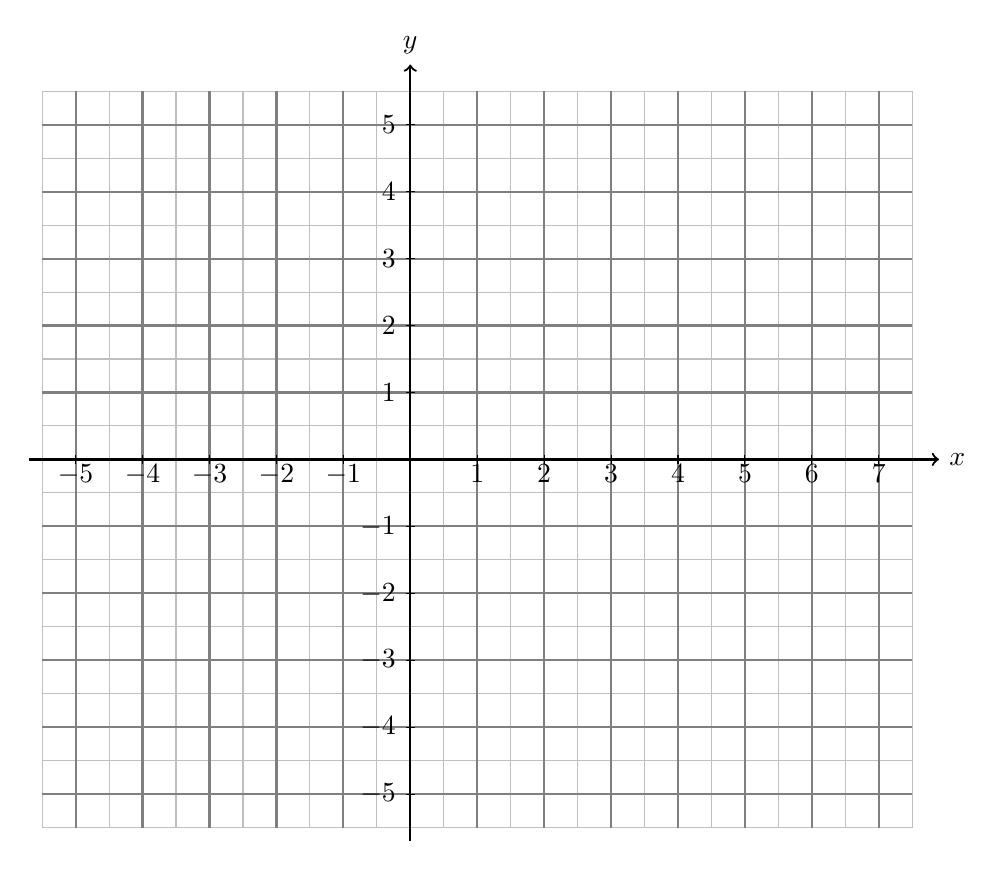
\begin{tikzpicture}[scale=0.85]

\draw [thin, color=lightgray, xstep=0.5cm, ystep=0.5cm] (-5.5,-5.5) grid (7.5,5.5);
\draw [thick, color=gray, xstep=1.0cm, ystep=1.0cm] (-5.5,-5.5) grid (7.5,5.5);

\foreach \x in {-5,-4,-3,-2,-1,1,2,3,4,5, 6, 7}
\draw[shift={(\x,0)}, color=black] (0pt,-2pt) -- (0pt,2pt) node[below] {$\x$};

\foreach \y in {-5,-4,-3,-2,-1,1,2,3,4,5}
\draw[shift={(0,\y)}, color=black] (2pt,0pt) -- (-2pt,0pt) node[left] {$\y$};

\draw [thick, ->] (-5.7,0) -- (7.9,0) node [right] {$x$};
\draw [thick, ->] (0,-5.7) -- (0,5.9) node [above] {$y$};

\end{tikzpicture}
\end{center}
\end{figure}

\newpage

%--- Problem 4: Translated reciprocal function ---
\item[4.] Consider the function
$\displaystyle g(x) = \dfrac{1}{x-2} + 1$.

\begin{enumerate}[label=(\alph*), itemsep=0.3cm]
  \item Write down the equations of the vertical and horizontal
  asymptotes of $g$.

  \vspace{1.4cm}

  \item Find the $y$-intercept of $g$.

  \vspace{1.6cm}

  \item Find the $x$-intercept of $g$.

  \vspace{1.8cm}

  \item Sketch the graph of $g$ on the axes below. Label the
  asymptotes (dashed) and the intercepts.
\end{enumerate}

\begin{figure}[H]
\begin{center}
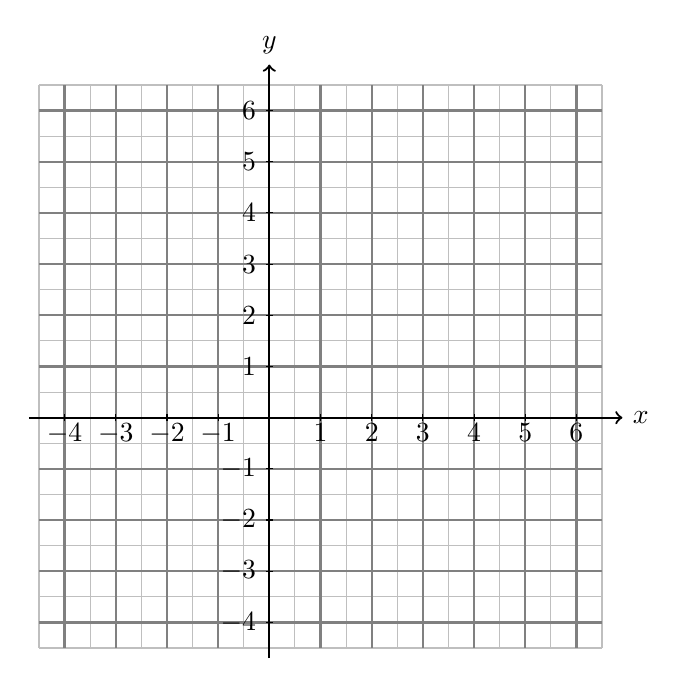
\begin{tikzpicture}[scale=0.65]

\draw [thin, color=lightgray, xstep=0.5cm, ystep=0.5cm] (-4.5,-4.5) grid (6.5,6.5);
\draw [thick, color=gray, xstep=1.0cm, ystep=1.0cm] (-4.5,-4.5) grid (6.5,6.5);

\foreach \x in {-4,-3,-2,-1,1,2,3,4,5,6}
\draw[shift={(\x,0)}, color=black] (0pt,-2pt) -- (0pt,2pt) node[below] {$\x$};

\foreach \y in {-4,-3,-2,-1,1,2,3,4,5,6}
\draw[shift={(0,\y)}, color=black] (2pt,0pt) -- (-2pt,0pt) node[left] {$\y$};

\draw [thick, ->] (-4.7,0) -- (6.9,0) node [right] {$x$};
\draw [thick, ->] (0,-4.7) -- (0,6.9) node [above] {$y$};

\end{tikzpicture}
\end{center}
\end{figure}

\newpage

%--- Problem 5: Derive the inverse of g(x) = 1/(x-2) + 1 ---
\item[5.] Let $g(x) = \dfrac{1}{x-2} + 1$, the function from
Problem 4.

\begin{enumerate}[label=(\alph*), itemsep=0.4cm]
  \item Find $g^{-1}(x)$. Show each step of your algebra.

  \vspace{5.5cm}

  \item Write down the equations of the vertical and horizontal
  asymptotes of $g^{-1}$.

  \vspace{1.6cm}

  \item Compare the asymptotes of $g$ (from Problem 4(a)) with the
  asymptotes of $g^{-1}$. What do you notice?

  \vspace{2.0cm}

  \item State the domain and range of $g^{-1}$.

  \vspace{1.4cm}
\end{enumerate}

\end{enumerate}
\end{document}
